\documentclass{article}
\usepackage{amsmath,amssymb}
\usepackage{tikz}
\usetikzlibrary{arrows,arrows.meta,backgrounds,calc,patterns,positioning,shapes,shadows}
\pgfdeclarelayer{bg}
\pgfsetlayers{bg,main}
\tikzset{
	arc/.style = {->, semithick, >={[round,sep]Stealth}},
	triangle/.style = {regular polygon, regular polygon sides = 3, inner sep = 0.5pt},
	failure/.style = {triangle, draw, fill = ibm3, minimum size = 0.5cm},
	component/.style = {ellipse, draw, fill = ibm5, minimum size = 0.6cm},
	function/.style = {rectangle, draw, fill = cyan!70, minimum size = 0.6cm},
	action/.style = {regular polygon, regular polygon sides = 5, draw, fill = ibm1, inner sep = 2pt, minimum size = 0.6cm},
	funcvar/.style = {ellipse, draw, fill = gray!15, minimum size = 0.6cm},
}

\begin{document}

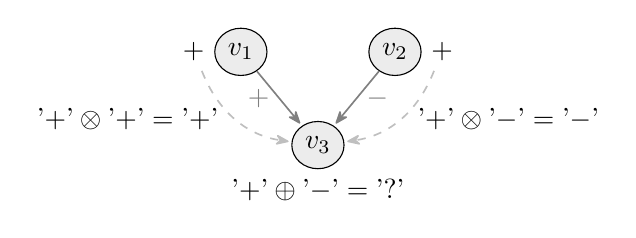
\begin{tikzpicture}
	\node[funcvar, align = center, inner sep = 2pt] (rv1) {$v_1$};
	\node[funcvar, align = center, inner sep = 2pt, below right = 0.75cm and 0.5cm of rv1] (rv3) {$v_3$};
	\node[funcvar, align = center, inner sep = 2pt, above right = 0.75cm and 0.5cm of rv3] (rv2) {$v_2$};

	\node[left = 0cm of rv1] (sign_rv1) {$+$};
	\node[right = 0cm of rv2] (sign_rv2) {$+$};
	\node[below = 0cm of rv3] (sign_rv3) {$\text{'$+$'} \oplus \text{'$-$'} = \text{'$?$'}$};

	\draw (rv1) edge[arc, gray] node[left] {$+$} (rv3);
	\draw (rv2) edge[arc, gray] node[right] {$-$} (rv3);

	\draw (sign_rv1) edge[arc, dashed, gray!50, bend right] node[black, left, xshift = -0.1cm] {$\text{'$+$'} \otimes \text{'$+$'} = \text{'$+$'}$} (rv3);
	\draw (sign_rv2) edge[arc, dashed, gray!50, bend left] node[black, right, xshift = 0.1cm] {$\text{'$+$'} \otimes \text{'$-$'} = \text{'$-$'}$} (rv3);
\end{tikzpicture}

\end{document}